\documentclass[conference]{IEEEtran}
\IEEEoverridecommandlockouts
% The preceding line is only needed to identify funding in the first footnote. If that is unneeded, please comment it out.
\usepackage{cite}
\usepackage{amsmath,amssymb,amsfonts}
\usepackage{algorithmic}
\usepackage{graphicx}
\usepackage{textcomp}
\usepackage{xcolor}
\usepackage[utf8]{inputenc}
\usepackage[english]{babel}
\usepackage{hyperref}

\urlstyle{same}
\def\BibTeX{{\rm B\kern-.05em{\sc i\kern-.025em b}\kern-.08em
    T\kern-.1667em\lower.7ex\hbox{E}\kern-.125emX}}
\begin{document}

\title{Human Activity Recognition(HAR)}



\author{\IEEEauthorblockN{ Vineeth Bhat}
\IEEEauthorblockA{\textit{Dept.Computer Science and Engineering} \\
\textit{Frankfurt University of Applied Sciences}\\
Frankfurt, Germany \\
vineeth.bhat@stud.fra-uas.de}
\and
\IEEEauthorblockN{Jathin Sreenivas}
\IEEEauthorblockA{\textit{Dept.Computer Science and Engineering} \\
\textit{Frankfurt University of Applied Sciences}\\
Frankfurt, Germany \\
Jahtin.Sreenivas@stud.fra-uas.de}
\and
\IEEEauthorblockN{Vidya Gopalakrishnarao}
\IEEEauthorblockA{\textit{Dept.Computer Science and Engineering} \\
\textit{Frankfurt University of Applied Sciences}\\
Frankfurt, Germany \\
vidya.gopalakrishnarao@stud.fra-uas.de}
}




\maketitle

\begin{abstract}
This document is an introduction to the project Human Activity Recognition(HAR). The scope of the project is to understand the working of the sensors in our smartphones or tablet and access it to track various human activity like walking, jogging, etc and propose a system(application) for the same.
\end{abstract}

\section{Project Vision}
Our smartphones are filled with sensors that read various data from the physical world around them. These data is then utilised by various application on the smartphone as per their need. The objective of this project is to provide an application that monitors the basic human activity with the help of sensors embedded in our smartphones. \\
We are building an application that access the sensors embedded in our smartphones are that are necessary to monitor the human activity and collect the data acquired by the sensor and present in it in a readable form to the user.

\section{Requirements}
\subsection{Functional Requirements}
\begin{itemize}
\item Primary requirement is to track the human activity using the appropriate sensors embedded in the smart phone
\item Accessing the sensor using the system's operating system to obtain the data.
\item Conversion sensor data into digital data.
\item Visualisation of data. That is representing the data collected in readable form.
\end{itemize}

\subsection{Non- Functional Requirements}
\begin{itemize}
\item Real time monitoring of human activity and displaying of collected data.
\item Accurate measurement of the activity by the sensor..
\item The application must adapt varying display sizes of mobile screen.
\item User friendly UI/UX.
\end{itemize}

\section{Security}
\begin{itemize}
\item Privacy of user information. Example location, login data.
\item Confidentiality of the data collected from the sensor.
\item Requesting access permission to monitor the activity and device features.
\item User authentication for accessing the app and data. 
\end{itemize}

\section{Reliability}
\begin{itemize}
\item The data collected from the sensor must be reliable for any further use.
\item Activity monitored must be accurate.
\item Capability to handle large amount of data and perform as intended.
\item State of the application is uninterrupted by external interruption.
\end{itemize}

\section{Development Environment}
As we are using android devices in our team we decided to do the project on android platform. For this we are considering the android studio as our development environment.\\
Using Android sensor framework we can access the available sensors and acquire the raw sensor data. Android provides dedicated hardware package for accessing the embedded sensors. It includes the following classes and interface, SensorManager, Sensor, SensorEvent, SensorEventListner.

\subsection{Sensors}

Android platform supports 3 categories of sensors,
\begin{itemize}
    \item Motion Sensors: These sensors are responsible for monitoring the acceleration force and rotational forces along the three axes. This category includes,gravity sensors, accelerometers, gyroscopes and rotational vector sensors.
    \item Position Sensors: Physical positioning of the device is measured b these sensors. These sensors include orientation sensors and magnetometer. 
    \item Environmental Sensors: Environmental parameters such as temperature, pressure, illumination and humidity are measured using these sensors. This includes, barometer, photometer and thermometer.
\end{itemize}

\subsection{Sensor Framework}

The sensor framework provides certain classes and interface to perform variety of sensor related tasks. For example, finding out the available sensors on the device. Figure.~\ref{fig1}. shows the list of available sensors on the android device that we intend to do this project on (Google Pixel 2). \\

\begin{figure}
\centerline{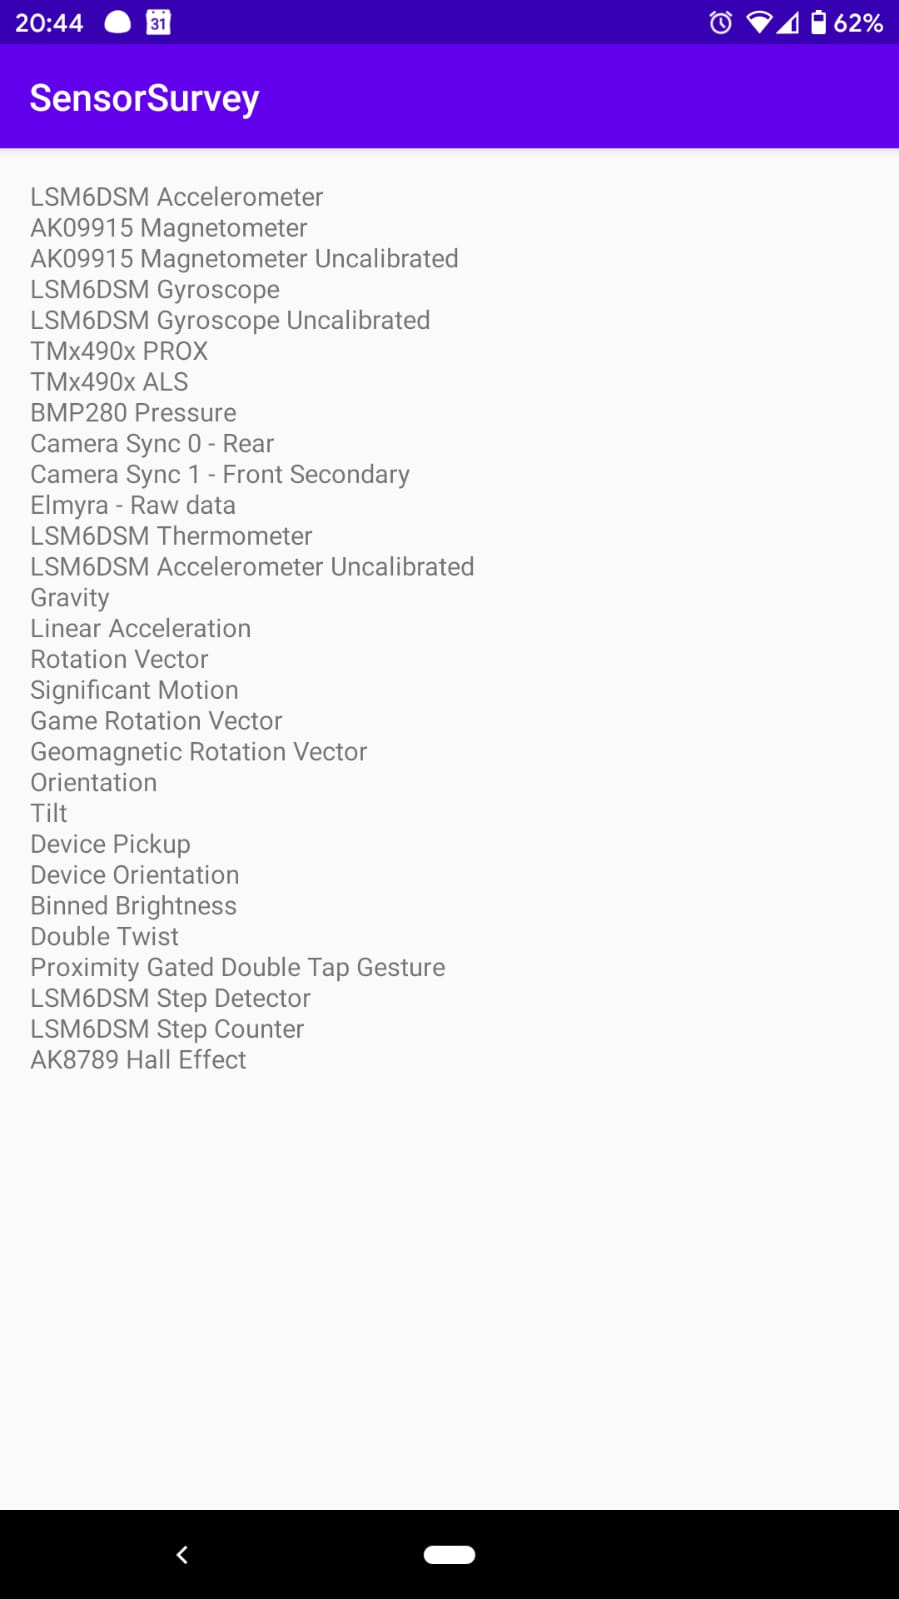
\includegraphics[width=8cm, height=11cm]{fig1.jpg}}
\caption{List of sensors embedded in Pixel 2.}
\label{fig1}
\end{figure}

The package that includes sensor framework is android.hardware. It provides following classes and interface to access the sensors,
\begin{itemize}
    \item SensorManager: This class is used to create an instance of the sensor service. It provides methods for accessing, listening and perform various action on the sensors.
    \item Sensor: This class is used to create an instance of a specific sensor.Sensor's capabilities are determined by this class.
    \item SensorEvent: Using this class the system creates a sensor event object, which is used to get information about the sensors. It inclde the following information, raw sensor data, type of the sensor that generated the event, timestamp, accuracy.
    \item SensorEventListener: Using this interface we can create two callback methods that receive notification when sensor values change or when sensor accuracy changes.
\end{itemize}
In a basic application we use these classes and interface to perform following tasks, identifying sensor and sensor capabilities and monitor sensoe events.

\subsection{Sensors Used}
There are various number of sensors that the android platform provides, for our project we'll be using the following sensors,\\
Accelerometer: Acceleration is the measurement of the rate of change in velocity, the accelerometer is an electromechanical device that is used for measuring acceleration forces. In the case of a sensor present in a mobile device, dynamic to sense movement or vibration. The accelerometer can operate in two ways the piezoelectric effect and the capacitance sensor. The Piezoelectric accelerometer uses microscopic crystal structures that become "squeezed" due to forces. These crystals create a voltage when squeezed and accelerometer interprets this voltage to determine the acceleration. Whereas the capacitance accelerometer changes the capacitance between microstructures located next to the device. If an accelerative force moves any of these structures the capacitance changes and accelerometer will read the capacitance and translates to a voltage for interpretation. In the android device the accelerometer measures the acceleration that is applied to a device on all three axes (x, y, and z), including the force of gravity. We are using this sensor to track the movement of the phone, and also to track the orientation and acceleration force of the device. In our application the acceleration along all the 3 axes in m2/s and the corresponding graph will be displayed, so if the phone is moved in any direction, the data and graph will change accordingly in real-time.\\
Gyroscope: The gyroscope sensor is a device that can measure and maintain the orientation and angular velocity of an object. They are more advanced than accelerometers. Accelerometers can measure only linear motion, whereas a gyroscope can measure tilt and lateral orientation. The Coriolis force concept is used in the Gyroscope sensors. To measure the angular rate, the rotation rate of the sensor is converted into an electrical signal. Measures a device's rate of rotation around each of the three physical axes (x, y, and z). A gyroscope can be used for navigation and measurement of angular velocity. In our application we will show the orientation along the three 3 axes in rad/s along with the corresponding graph.\\
Magnetometer: The Magnetometer sensor reads the strength of the magnetic field around an Android device.The sensors measure the physical position of a device which reports the ambient magnetic  field, sensor produces  voltage which is proportional to the strength and polarity of the magnetic field along the axis each sensor is directed. The sensed voltage is converted to digital signal representing the magnetic field intensity. Magnetic field measured along the three sensor axes  x, y, and z fields of “sensors\_even\_t.magnetic” and all values are in micro-Tesla(μT).

\begin{thebibliography}{00}
\bibitem{b1} https://developer.android.com/guide/topics/sensors Accessed: 26.05.2020
\bibitem{b2} https://ef.engr.utk.edu/hyperphysics/hbase/gyr.html Accessed: 26.05.2020
\bibitem{b3} https://www.livescience.com/40102-accelerometers.html Accessed: 26.05.2020
\end{thebibliography}
\vspace{12pt}

\end{document}
